% Especificaciones del tamaño de letra, tamaño de hoja, márgenes, librerias, etc.
\documentclass[12pt, letterpaper]{article}
\usepackage[english]{babel}
\usepackage{fancyhdr}
\usepackage[utf8]{inputenc}
\usepackage[T1]{fontenc}
\usepackage{amsmath}
\usepackage{graphicx}
\usepackage{subcaption}
\usepackage[hidelinks]{hyperref}
\usepackage{url}
\usepackage{amssymb}
\usepackage{float}
\usepackage[margin=1in]{geometry}
\renewcommand{\baselinestretch}{1.5}

% Enlace Bibliografía
\usepackage{csquotes}
\usepackage[notes,backend=biber]{biblatex-chicago}
\addbibresource{referencias.bib}

% Titulo, autores, fecha.
\title{Práctica \#9: Análisis de Torsión para Pieza Sólida y Hueca}
\author{Carlos Vásquez \and 1155057}
\date{May 9, 2019}
\pagestyle{fancy}
\fancyhf{}
\rhead{Carlos Vásquez}
\lhead{Práctica \#9}
\rfoot{\thepage}


% Inicio del documento
\begin{document}
\maketitle
\section*{Introducción}
Para esta práctica nos enfocaremos en el análisis de torsión que pueden soportar las distintas barras, y posteriormente compararemos estas torsiones y sus pesos.

Mostraremos el análisis hecho en SOLIDWORKS y después se mostrarán las ecuaciones utilizadas de manera teórica para obtener resultados similares a aquellos que nos brinda el programa.

\section*{Desarrollo}
Ambas barras que se analizarán tiene el mismo diámetro externo de $4\ in$, sin embargo la barra hueca tiene un diámetro interior de $2\ in$, lo cual le retira bastante peso a ésta. La extrusión realizada fue de $12\ in$.

El esfuerzo máximo admisible es de $10000 \frac{lb}{in^2}$. Teniendo estas restricciones en cuenta, podemos analizar los resultados que hemos obtenido de SOLIDWORKS.

\begin{figure}[H]
	\centering
	\begin{subfigure}[b]{0.49\linewidth}
		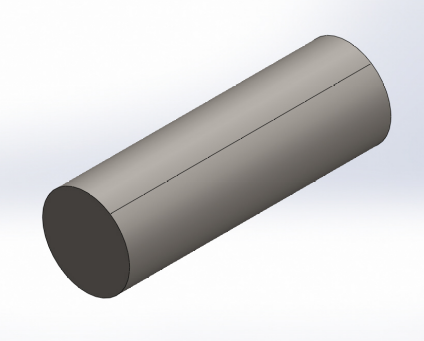
\includegraphics[width=\linewidth]{s.png}
		\caption{Barra sólida}
	\end{subfigure}
	\begin{subfigure}[b]{0.49\linewidth}
		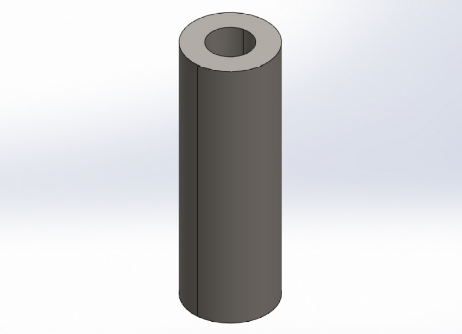
\includegraphics[width=\linewidth]{h.png}
		\caption{Barra hueca.}
	\end{subfigure}
	\caption{Los diámetros externos son de $4\ in$ y ambas soportarán un esfuerzo admisible de $10000 \frac{lb}{in^2}$}
\end{figure}


\begin{figure}[H]
	\centering
	\begin{subfigure}[b]{0.49\linewidth}
		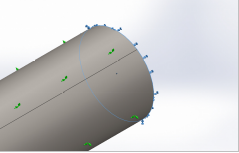
\includegraphics[width=\linewidth]{suj1.png}
		\caption{Sujeción fija.}
	\end{subfigure}
	\begin{subfigure}[b]{0.49\linewidth}
		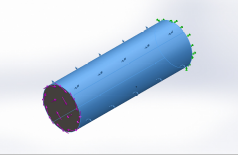
\includegraphics[width=\linewidth]{suj2.png}
		\caption{Sujeción sobre cara cilíndrica.}
	\end{subfigure}
	\caption{Sujeciones en la pieza sólida.}
\end{figure}


\begin{figure}[H]
	\centering
	\begin{subfigure}[b]{0.49\linewidth}
		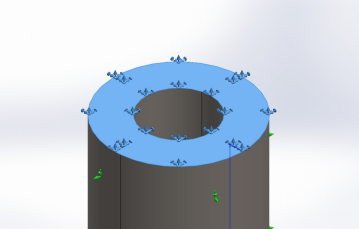
\includegraphics[width=\linewidth]{suj3.png}
		\caption{Sujeción fija.}
	\end{subfigure}
	\begin{subfigure}[b]{0.49\linewidth}
		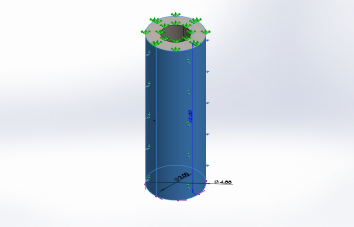
\includegraphics[width=\linewidth]{suj4.png}
		\caption{Sujeción sobre cara cilíndrica.}
	\end{subfigure}
	\caption{Sujeciones en la pieza hueca.}
\end{figure}


\begin{figure}[H]
	\centering
	\begin{subfigure}[b]{0.49\linewidth}
		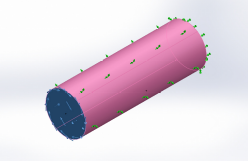
\includegraphics[width=\linewidth]{c1.png}
		\caption{Carga en la pieza sólida.}
	\end{subfigure}
	\begin{subfigure}[b]{0.49\linewidth}
		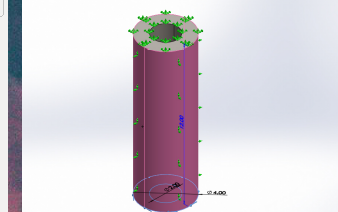
\includegraphics[width=\linewidth]{c2.png}
		\caption{Carga en la pieza hueca.}
	\end{subfigure}
	\caption{Las cargas en ambas piezas son distintas, sin embargo cada una produce un esfuerzo cortante de 10,000 psi.}
\end{figure}


\begin{figure}[H]
	\centering
	\begin{subfigure}[b]{0.49\linewidth}
		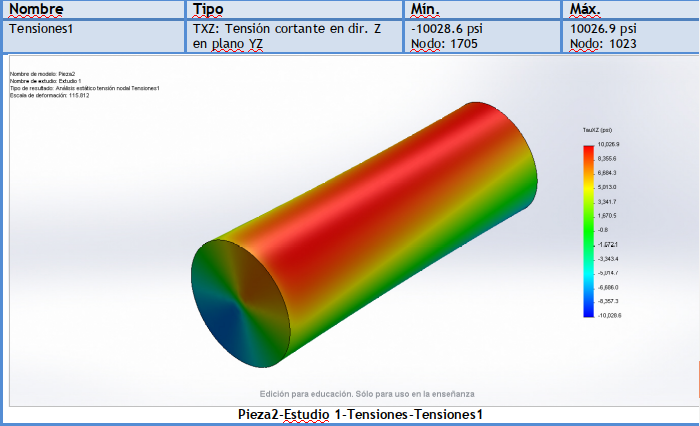
\includegraphics[width=\linewidth]{r1.png}
		\caption{Resultados de la pieza sólida.}
	\end{subfigure}
	\begin{subfigure}[b]{0.49\linewidth}
		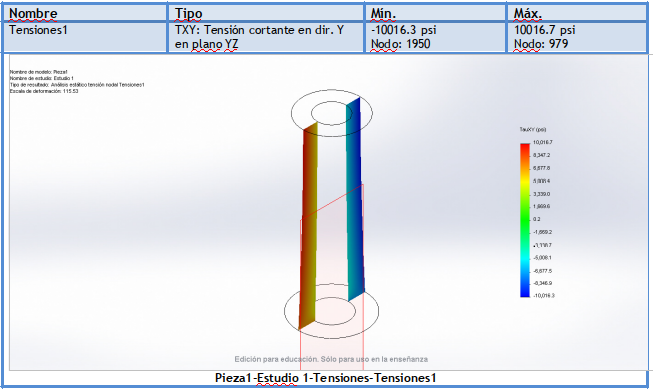
\includegraphics[width=\linewidth]{r2.png}
		\caption{Resultados de la pieza hueca.}
	\end{subfigure}
	\caption{Podemos observar que el esfuerzo cortante es aproximadamente 10,000 psi.}
\end{figure}

\section*{Cálculos}

Para encontrar la manera en la que se relacionan estas piezas, podemos realizar un análisis de torsión. Dado que conocemos los diámetros de ambas piezas y los esfuerzos cortantes admisibles, podemos calcular el par torcional que se está aplicando a cada pieza. Nos referiremos a todos aquellos resultados de la pieza sólida con el subíndice 1 y a todos los resultados de la pieza hueca con el subíndice 2.

Por lo tanto, para calcular el par torsional podemos hacer uso de las siguientes fórmulas:

\begin{equation}
	J = \frac{\pi D^4}{32}
\end{equation}
\begin{equation}
	\tau = \frac{Tc}{J}
\end{equation}

Si utilizamos las ecuaciones (1) y (2) con los datos de la pieza sólida y despejamos para obtener $T$ obtenemos

\begin{equation}
	T_1 = \frac{J_1 \tau_1}{c_1} = \boxed{125663.7\ lb \cdot in}
\end{equation}

De la misma manera podemos obtener el par torsional que actúa en la pieza hueca, sin embargo el momento polar de inercia ($J$) cambia un poco dado que ya no contamos con una barra totalmente sólida. Para $J_2$ tendremos

\begin{equation}
	J_2 = \frac{\pi (D_E^4 - D_I^4)}{32}
\end{equation}
\begin{center}
	Donde $D_E$ es el diámetro externo y $D_I$ el diámetro interno.
\end{center}

Por lo tanto, para calcular $T_2$ Debemos utilizar la ecuación (2) y (4). Por tanto

\begin{equation}
	\boxed{T_2 = 117809.7245\ lb\cdot in}
\end{equation}

Una vez hechos estos cálculos, para hacer nuestra comparación entre $T_1$ y $T_2$ podemos asumir que $T_1 \propto T_2$, o, en otras palabras, podemos decir que

\begin{equation}
	T_1 = \alpha T_2
\end{equation}

$T_2$ es $\alpha$ veces $T_1$. Entonces, si realizamos ese cálculo y despejamos $\alpha$ obtenemos

\begin{equation}
	\alpha = \frac{T_1}{T_2} = 0.9375 = 93.75 \%
\end{equation}
A partir del resultado de la ecuación (7), llegamos a la conclusión de que el par torsional $T_2$ es casi el mismo que $T_1$, teniendo una diferencia del $6.26\%$. Podrá parecer poca la diferencia pero con pares de torsión tan grande es más considerable esta diferencia absoluta y se vuelve más alarmante. Sin embargo, veamos cuál es la ganancia o diferencia en peso entre la barra sólida y la barra hueca.

Para comparar los pesos de estas barras podemos asumir, de la misma manera que con los pares torsionales, que $P_2 \propto P_1$, por lo tanto

\begin{equation}
	\begin{split}
		P_2 &= \beta P_1\\
		\beta &= \frac{P_2}{P_1}
	\end{split}
\end{equation}

Esto lo podemos entender físicamente como: "\textit{el peso de la barra hueca es $\beta$ veces el peso del peso de la barra sólida.}"
Desarrollando más la ecuación (8) obtenemos

\begin{equation}
	\begin{split}
		\beta &= \frac{A_2 l_1 \rho_2 g}{A_1 l_2 \rho_1 g}
	\end{split}
\end{equation}
\begin{center}
	Donde A representa el área de la sección transversal de cada una de las barras, l la longitud de cada barra, $\rho$ representa la densidad del material y g la constante gravitatoria. 
\end{center}
Dado que el material en ambas barras es el mismo y la longitud también podemos simplificar la ecuación.
\begin{equation}
	\begin{split}
		\beta &= \frac{A_2 l \rho g}{A_1 l \rho g}\\
		\beta &= \frac{A_2}{A_1}\\
		\beta &= \frac{3}{4}
	\end{split}
\end{equation}

Como observamos en la ecuación (10), y como anteriormente habíamos remarcado, podemos decir que \textit{el peso de la barra hueca es tres cuartos el peso de la barra sólida}, disminuyendo significativamente el peso. Esto es importante, porque con una disminucción del $0.75\%$ obtuvimos un par torsional que se asemeja en un $93.75\%$. Esto abre un gran espacio para la ingeniería al momento de diseñar ejes para transmitir potencia, ya que es posible reducir considerablemente el peso de éstos sin tener que sacrificar una gran cantidad de par torsional y, por defecto, esfuerzo admisible en la barra.

\section*{Conclusión}

Al analizar los pesos y los pares de torsión nos percatamos de que los ejes huecos, a pesar de tener una pérdida mínima de par torsional, éstos hacen que valga la pena esta pérdida ddebido a lo que ahorra en peso. Esto es una gran ventaja desde el punto de vista de la ingeniería dado que la libertad para diseñar ejes ha aumentado considerablemente con estos resultados. Sin embargo tenemos que estar conscientes que, cuando trabajamos con números muy grandes, estos porcentajes pueden cambiar o, en medidas absolutas, pueden ser diferencias mucho más grandes.

Es por esto que, dependiendo de la aplicación que le demos a estos ejes, entonces tomaremos la decisión más conveniente. Debemos evaluar si necesitaoms ahorar un gran peso o si debemos retener esa capacidad de soportar tal par torsional.
%%%%%  Bib
\renewcommand\refname{Referencias}
\printbibliography
\end{document}
